\documentclass[11pt]{beamer}
\usetheme{Madrid}
\usepackage[utf8]{inputenc}

\usepackage[OT2]{fontenc}
\usepackage[serbianc, serbian]{babel}
\usepackage{graphicx}


\title{Informacioni sistem za menad2ment transporta shec1era u Republici Srbiji}

\newcommand{\email}{email}


\setbeamertemplate{navigation symbols}{} 
\logo{
\includegraphics[scale=0.08]{Slike/Prezentacija/matfLogo.png}} 
\institute[]{Matematichki fakultet \\ Univerzitet u Beogradu} 
\date{\today} 
%\subject{}

% ---------------------------------------------------------
% Selecione um estilo de referência
\bibliographystyle{plain}

%\bibliographystyle{abbrv}
%\setbeamertemplate{bibliography item}{\insertbiblabel}
% ---------------------------------------------------------

% ---------------------------------------------------------
% Incluir os slides nos quais as referências foram citadas
%\usepackage[brazilian,hyperpageref]{backref}

%\renewcommand{\backrefpagesname}{Citado na(s) página(s):~}
%\renewcommand{\backref}{}
%\renewcommand*{\backrefalt}[4]{
%	\ifcase #1 %
%		Nenhuma citação no texto.%
%	\or
%		Citado na página #2.%
%	\else
%		Citado #1 vezes nas páginas #2.%
%	\fi}%
% ---------------------------------------------------------

\begin{document}
%--------------------------------------------------------%
\begin{frame}
\titlepage
\end{frame}
%--------------------------------------------------------%

\begin{frame}{Sadrzhaj}
\tableofcontents 
\end{frame}
%--------------------------------------------------------%
\section{Uvod}
%--------------------------------------------------------%
\begin{frame}{Uvod}
\begin{itemize}
    \item U Srbiji, trzhishte shec1era se procenjuje na 45 miliona americhkih dolara.

\end{itemize}
\end{frame}
%--------------------------------------------------------%
\begin{frame}{Uvod}
\begin{itemize}
    \item U Srbiji, trzhishte shec1era se procenjuje na 45 miliona americhkih dolara.
    \item U lancu nabavke shec1era, transport predstavlja najskuplju komponentu.

\end{itemize}
\end{frame}
%--------------------------------------------------------%
\begin{frame}{Uvod}
\begin{itemize}
    \item U Srbiji, trzhishte shec1era se procenjuje na 45 miliona americhkih dolara.
    \item U lancu nabavke shec1era, transport predstavlja najskuplju komponentu.

    \item Razvijen informacioni sistem za transportno preduzec1e.
\end{itemize}
\end{frame}
%--------------------------------------------------------%
\section{Analiza sistema}
%--------------------------------------------------------%

\begin{frame}{Opis procesa transporta}
    \begin{itemize}
    
    \item  Transport se vrshi od fabrike do magacina klijenta, po narud2bini.
    \item Narud2bine se vrshe na veliko.
    \item Klijenti su prehrambeni proizvodjachi.
    
    \end{itemize}
    
\end{frame}
%--------------------------------------------------------%
\begin{frame}{Opis procesa transporta}
    
    \begin{enumerate}
        \item Klijent naruchuje shec1er.
        \item Vrshi se utovar u kamione.
        \item Vrshi se transport.
        \item Vozach se vrac1a u fabriku.
    \end{enumerate}

    Jedan vozach opsluzhuje jednog klijenta i vrac1a se u fabriku.
\end{frame}
%--------------------------------------------------------%
\begin{frame}{Zahtevi klijenta}
    
    \begin{enumerate}
        \item Brza dostava.
        \item Bez kashnjenja.
        \item Shto jeftinije.
    \end{enumerate}
\end{frame}
%--------------------------------------------------------%
\begin{frame}{Zahtevi transportnog preduzec1a}
    
    \begin{enumerate}
        \item Brza i precizna obrada zahteva.
        \item Reagovanje na promene tokom transporta.
        \item Zadovoljni klijenti.
    \end{enumerate}
\end{frame}
%--------------------------------------------------------%
\begin{frame}{Uchesnici u sistemu}
    
    \begin{enumerate}
        \item Administratori
        \item Logistichari
    \end{enumerate}
\end{frame}
%--------------------------------------------------------%
\begin{frame}{Uchesnici u sistemu}
    
    \begin{enumerate}
        \item Administratori
        \item Logistichari
        \bigskip
        \item Klijenti
    \end{enumerate}
\end{frame}
%--------------------------------------------------------%
\begin{frame}{Uchesnici u procesu}
    
    \begin{enumerate}
        \item Administratori
        \item Logistichari
        \bigskip
        \item Klijenti
        \bigskip
        \item Vozachi
        \item Magacioneri
        \item Najamnici
        \item Serviseri
    \end{enumerate}
\end{frame}
%--------------------------------------------------------%

\section{Sluchajevi upotrebe}

\begin{frame}{Sluchajevi upotrebe}
    Sluchajevi upotrebe su grupisani u 3 kategorije:
    
    \begin{itemize}
        \item Administrativni poslovi
        \item Logistika i transport
        \item Odrzhavanje vozila
    \end{itemize}
    
\end{frame}
%--------------------------------------------------------%
\subsection{Administrativni poslovi}
%--------------------------------------------------------%
\begin{frame}{Administrativni poslovi}
\begin{itemize}
    \item Uchesnik je administrator sistema.
    \item Administrator upravlja podacima o klijentima.
\end{itemize}
\end{frame}
%--------------------------------------------------------%
\begin{frame}{Administrativni poslovi - dijagram}
\begin{figure}
    \centering
    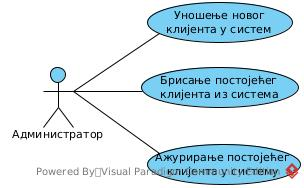
\includegraphics[scale=0.8]{Slike/UML/SUadministrativniPoslovi.jpg}
    \caption{Sluchaj upotrebe: Administrativni poslovi}
\end{figure}
\end{frame}
%--------------------------------------------------------%
\begin{frame}{Administrativni poslovi - BPMN dijagram}
\begin{figure}
    \centering
    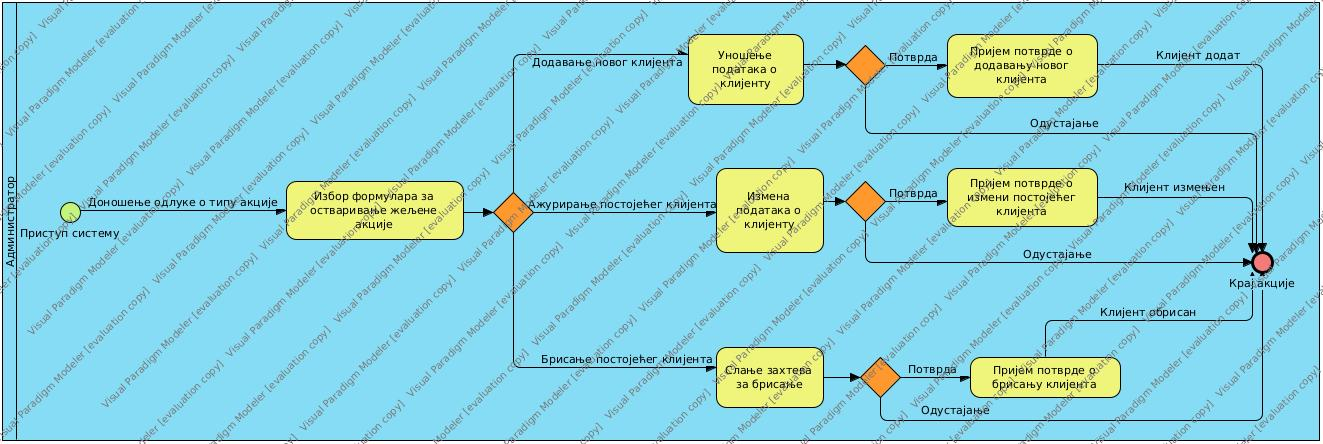
\includegraphics[scale=0.25]{Slike/BPMN/BPMNadministrativniPoslovi.jpg}
    \caption{BPMN: Administrativni poslovi}
\end{figure}
\end{frame}
%--------------------------------------------------------%
% \begin{frame}{Administrativni poslovi - dijagram}
% \begin{figure}
%     \centering
%     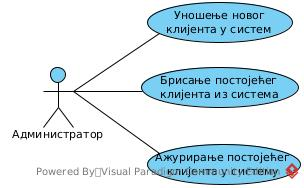
\includegraphics[scale=0.8]{Slike/UML/SUadministrativniPoslovi.jpg}
%     \caption{Sluchaj upotrebe: Administrativni poslovi}
%     \label{fig:ap}
% \end{figure}
% \end{frame}

\subsection{Logistika i transport}
%--------------------------------------------------------%
\begin{frame}{Logistika i transport}
   \begin{itemize}
       \item Proces planiranja transporta.
       \item Utovar.
       \item Realizacija transporta.
       \item Naplata.
   \end{itemize}

\end{frame}
%--------------------------------------------------------%
\begin{frame}{Planiranje transporta}
   
TODO...
\end{frame}
%--------------------------------------------------------%
\begin{frame}{Dostava porud2bine}
   

\end{frame}
%--------------------------------------------------------%
\begin{frame}{Dostava porud2bine - dijagram}
\begin{figure}
    \centering
    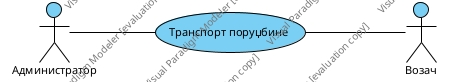
\includegraphics[scale=0.6]{Slike/UML/SUdostavljanjePorudzbineUseCase.jpg}
    \caption{Sluchaj upotrebe: Dostava porud2bine}
    \label{fig:dp}
\end{figure}
\end{frame}
%--------------------------------------------------------%
\begin{frame}{Dostava porud2bine - dijagram aktivnosti}
\begin{figure}
    \centering
    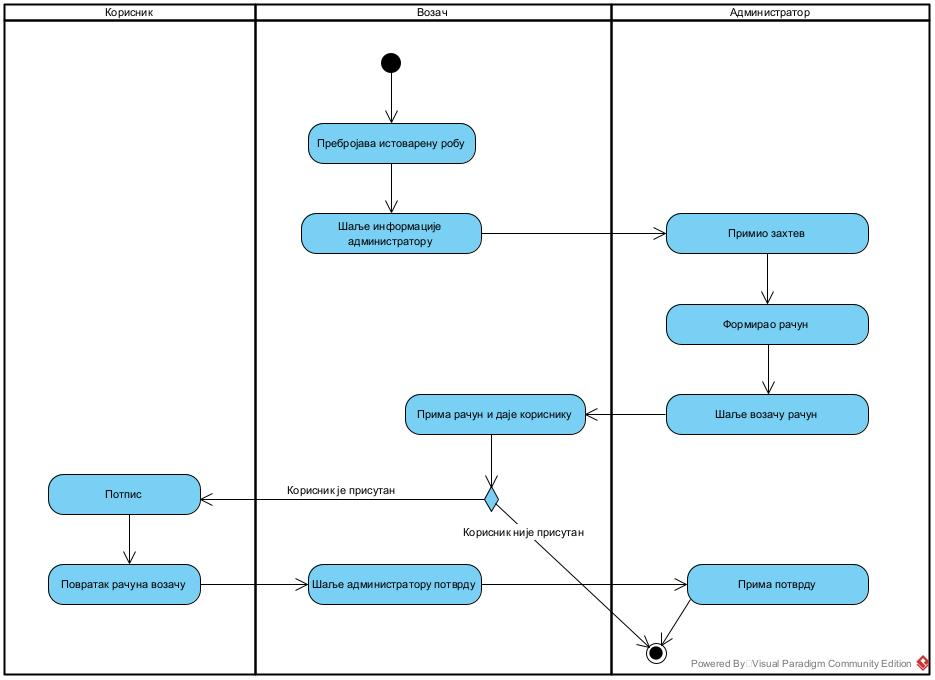
\includegraphics[scale=0.23]{Slike/DFD/AD_transport.jpg}
    \caption{Dijagram aktivnosti: Dostava porud2bine}
    \label{fig:dadp}
\end{figure}
\end{frame}
%--------------------------------------------------------%
\begin{frame}{Dostava porud2bine - dijagram sekvenci}
\begin{figure}
    \centering
    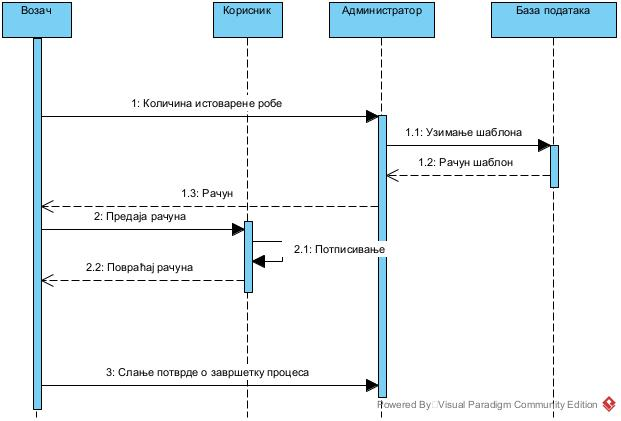
\includegraphics[scale=0.4]{Slike/DFD/DS_transport.jpg}
    \caption{Dijagram sekvenci: Dostava porud2bine}
    \label{fig:dsdp}
\end{figure}
\end{frame}
%--------------------------------------------------------%
\begin{frame}{Dostava porud2bine - BPMN dijagram}
\begin{figure}
    \centering
    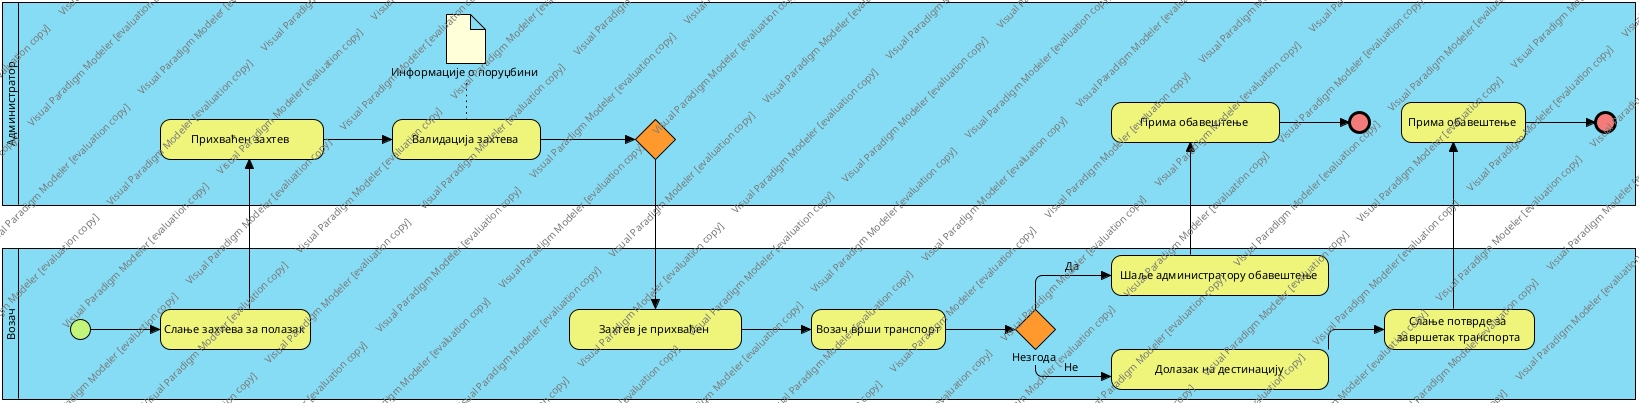
\includegraphics[scale=0.19]{Slike/BPMN/SUdostavljanjePorudzbineBPMN.jpg}
    \caption{Dijagram aktivnosti: Dostava porud2bine}
    \label{fig:bmpndp}
\end{figure}
\end{frame}
%--------------------------------------------------------%
\begin{frame}{Zavrshna faza porud2bine}
\begin{figure}
    \centering
    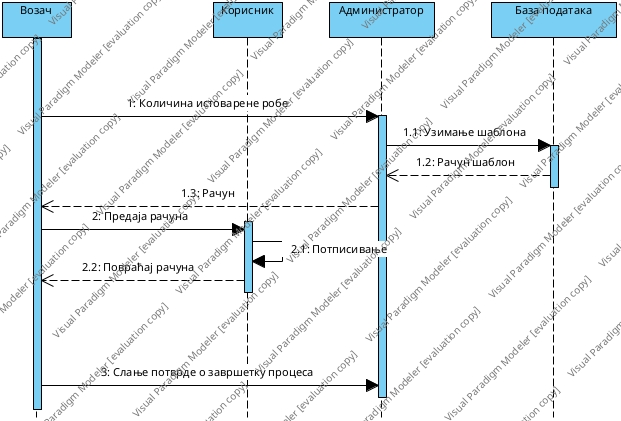
\includegraphics[scale=0.4]{Slike/DFD/SUzavrsnaFazaProudzbineSequence Diagram1.jpg}
    \caption{Dijagram sekvenci: Zavrshna faza}
    \label{fig:dsfzp1}
\end{figure}
\end{frame}
%--------------------------------------------------------%
\begin{frame}{Zavrshna faza porud2bine - dijagram}
\begin{figure}
    \centering
    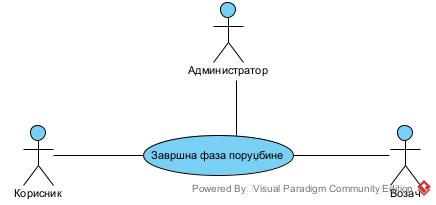
\includegraphics[scale=0.4]{Slike/UML/SUzavrsnaFaza.jpg}
    \caption{Sluchaj upotrebe: Zavrshna faza porud2bine}
    \label{fig:suzfp}
\end{figure}
\end{frame}
%--------------------------------------------------------%
\begin{frame}{Zavrshna faza porud2bine - BPMN dijagram}
\begin{figure}
    \centering
    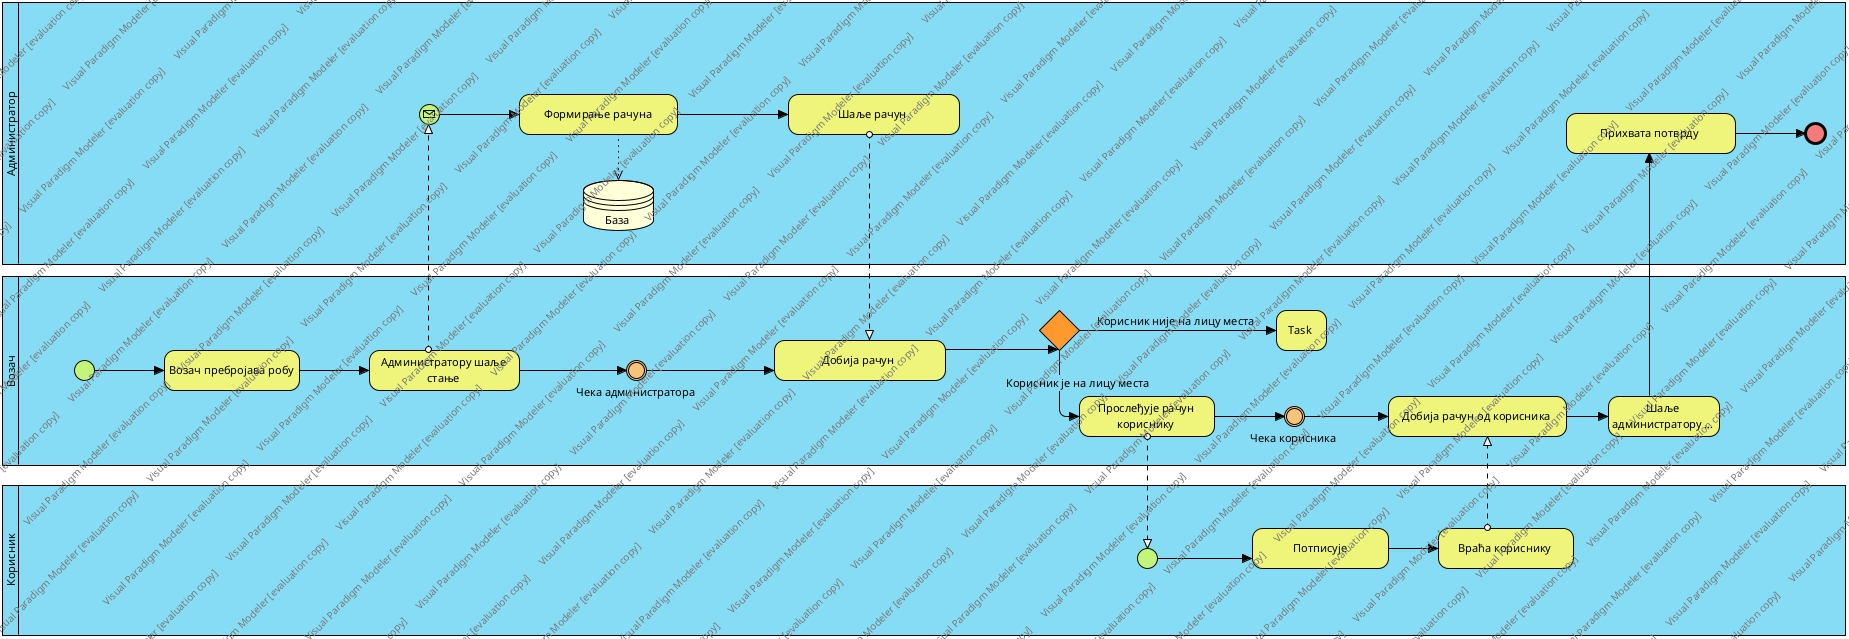
\includegraphics[scale=0.17]{Slike/BPMN/BPMNzavrsnaFazaPorudzbine.jpg}
    \caption{BPMN dijagram: Zavrshna faza porud2bine}
    \label{fig:bpmnzfp}
\end{figure}
\end{frame}
%--------------------------------------------------------%
\begin{frame}{Zavrshna faza porud2bine - dijagram sekvenci}
\begin{figure}
    \centering
    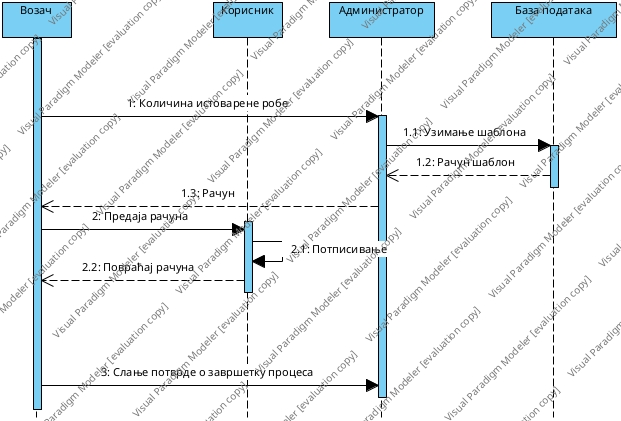
\includegraphics[scale=0.4]{Slike/DFD/SUzavrsnaFazaProudzbineSequence Diagram1.jpg}
    \caption{Dijagram sekvenci: Zavrshna faza porud2bine}
    \label{fig:dszfp}
\end{figure}
\end{frame}
%--------------------------------------------------------%
\subsection{Odrzhavanje vozila}
%--------------------------------------------------------%

\begin{frame}{Odrzhavanje vozila}
    \begin{itemize}
        \item Prijava kvara.
        \item Unoshenje novih vozila u sistem 
        \item Brisanje vozila iz sitema
        \item Az1uriranje vozila u sistemu
    \end{itemize}
    Uchesnici su vozach i serviser. Serviser upravlja podacima o vozilima i bavi se reorganizacijom transporta u sluchaju kvara na putu.
\end{frame}
%--------------------------------------------------------%
\begin{frame}{Odrzhavanje vozila - dijagram}
    \begin{figure}
        \centering
        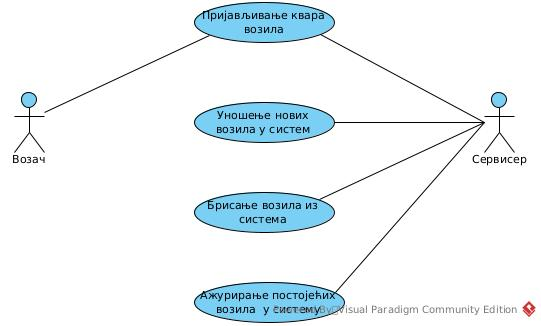
\includegraphics[scale=0.6]{Slike/UML/SUodrzavanje.jpg}
        \caption{Sluchaj upotrebe: Odrzhavanje vozila}
        \label{fig:ov}
    \end{figure}    
\end{frame}
%--------------------------------------------------------%
\begin{frame}{Odrzhavanje vozila - BPMN dijagram}
    \begin{figure}
        \centering
        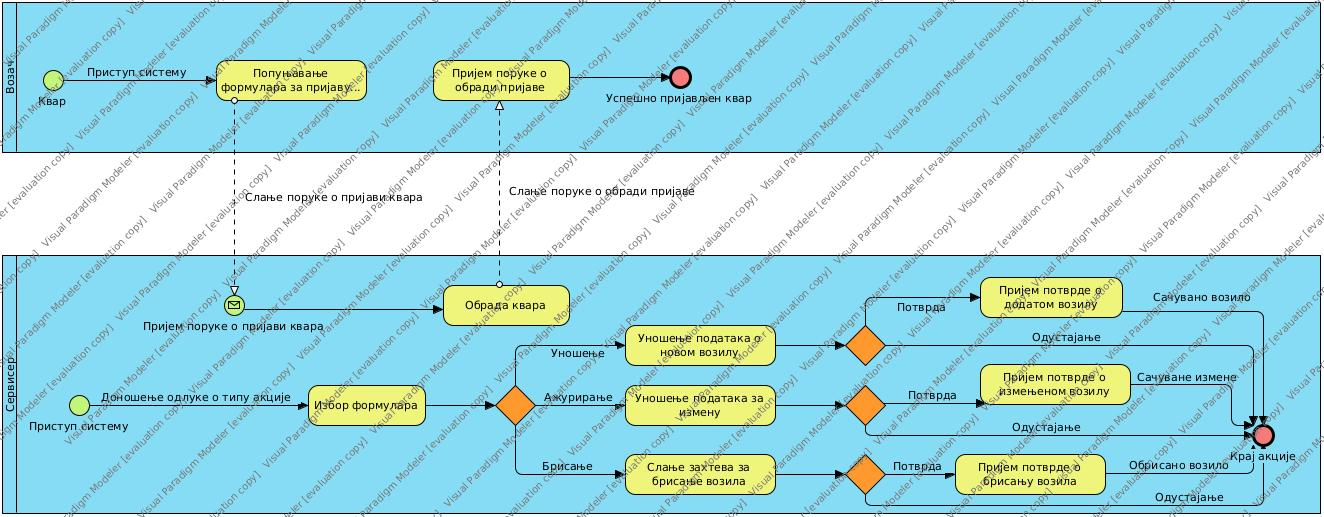
\includegraphics[scale=0.25]{Slike/BPMN/BPMNodrzavanje.jpg}
        \caption{BPMN dijagram: Odrzhavanje vozila}
        \label{fig:bpmnov}
    \end{figure}    
\end{frame}
%--------------------------------------------------------%

\section{Model baze podataka}
%--------------------------------------------------------%
\begin{frame}{Model baze}
TODO...
\end{frame}
%--------------------------------------------------------%

\section{Predlog arhitekture sistema}
%--------------------------------------------------------%
\begin{frame}{Karakteristike arhitekture}
 Jednostavna, stabilna, bezbedna, sirokodostupna aplikacija.
Karakteristike:
\begin{enumerate}
    \item Tip aplikacije: veb aplikacija.
    \item Strategija isporuchivanja: jedan serverski i vishe klijentskih rachunara.
    \item Tehnologije: $HTML, CSS, PHP, Javascript$
    \item Pratec1e komponente:
    \begin{itemize}
        \item Logovanje na sistem: Podsistem za autentikaciju korisnika.
        \item Pomoc1: Uputstvo za korish\-c1enje, $FAQ.$
        \item Pravljenje kopije baze podataka.
    \end{itemize}
    
\end{enumerate}
\end{frame}
%--------------------------------------------------------%
\begin{frame}{Predlog arhitekture - dijagram}
 \begin{figure}
     \centering
     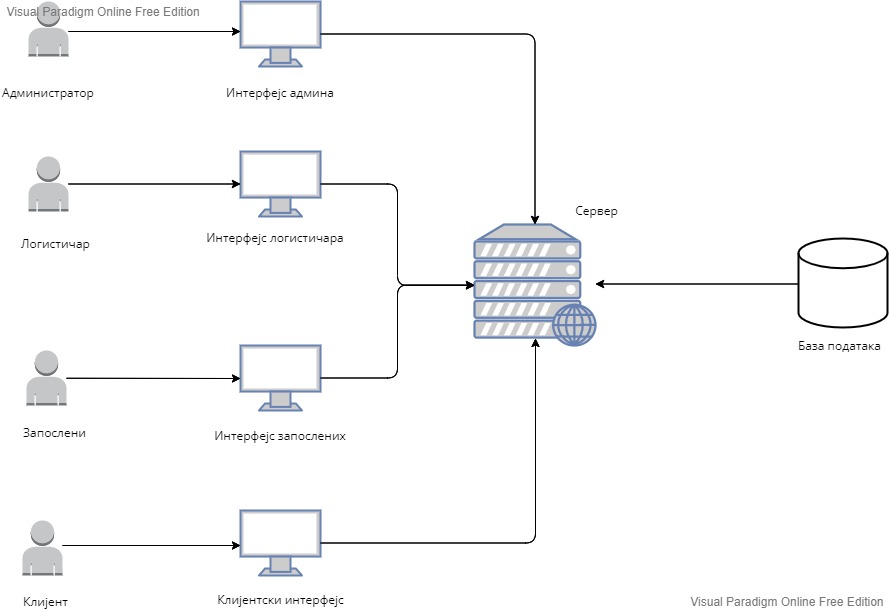
\includegraphics[scale=0.25]{Slike/Arhitektura/arhitektura .jpg}
     \caption{Predlog arhitekture}
 \end{figure}
 \end{frame}
%--------------------------------------------------------%
\begin{frame}{Tip i slojevi arhitekture}
Klijent-server arhitektura sa tri sloja:
\begin{enumerate}
    \item Prezentacioni sloj
    \item Logichki sloj
    \begin{itemize}
        \item Klijent kontroler
        \item Server kontroler
    \end{itemize}
    \item Sloj podataka
\end{enumerate}
 \end{frame}
%--------------------------------------------------------%
\begin{frame}{Predlog arhitekture - dijagram}
    \begin{figure}
        \centering
        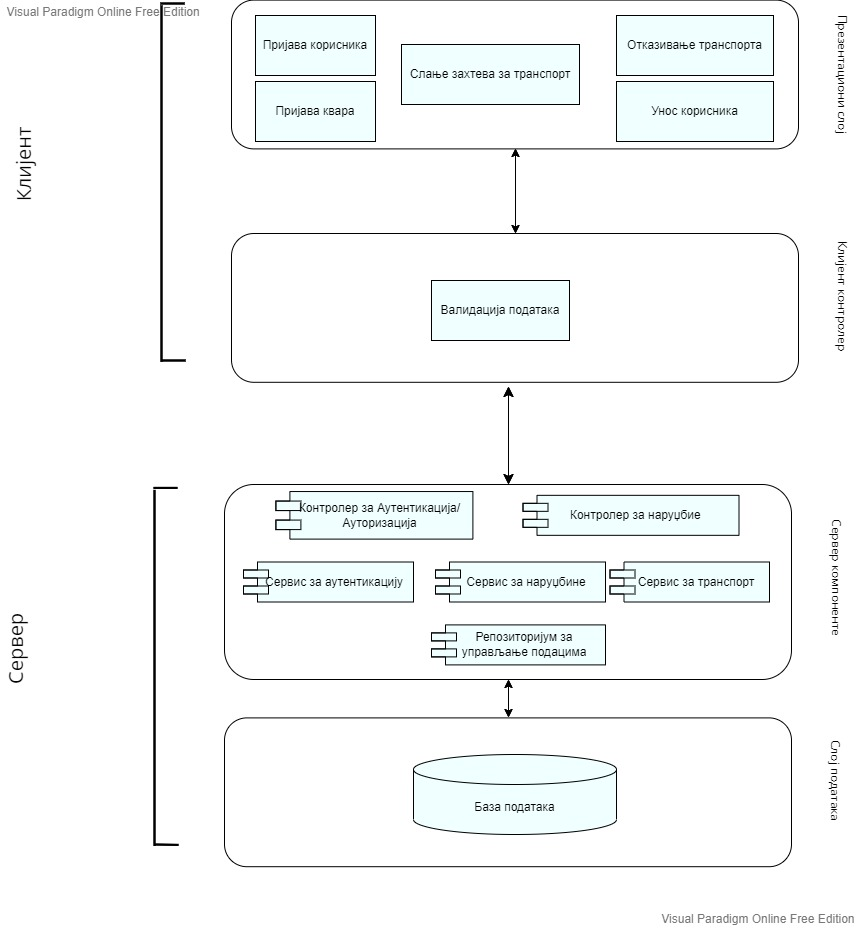
\includegraphics[scale=0.20]{Slike/Arhitektura/predlogArhitekture.jpg}
        \caption{Klijent server arhitektura}
        \label{fig:ksa}
    \end{figure}
 \end{frame}
%--------------------------------------------------------%

\section{Korisnichki interfejs}
%--------------------------------------------------------%


%--------------------------------------------------------%
\section{Zakljuchak}
%--------------------------------------------------------%
\begin{frame}{Zakljuchak}
    \begin{itemize}
        \item Razvijen informacioni sistem za transportno preduzec1e.
        \item Opisane funkcionalnosti za funkcionisanje sistema.
        \item Predlozhen relacioni model baze podataka.
        \item Predlozhena klijent-server arhitektura.
    \end{itemize}
\end{frame}
%--------------------------------------------------------%

\begin{frame}{Dalji razvoj sistema}
    \begin{itemize}
        \item Proshirivanje na inostrani transport.
        
        \medskip
        
        \item Uvodjenje periodichnih nabavki.
        
        \medskip
        \item Prac1enje poshiljke.
        \medskip
        \item Omoguc1avanje manjih nabavki.
    \end{itemize}
\end{frame}
%--------------------------------------------------------%

\section{Literatura}
%--------------------------------------------------------%

\begin{frame}{Literatura}
    \bibliography{literatura}
    \begin{itemize}
        \item{\textit{Informacioni sistem za menad2ment transporta shec1era u Republici Srbiji}, Marija Eric1, Milosh Kutleshic1, Milica Gajic1}
    \end{itemize}
    
\end{frame}
%--------------------------------------------------------%

\begin{frame}
\begin{center}
    Hvala na pazhnji!
\end{center}
%--------------------------------------------------------%

\end{frame}

\end{document}